\documentclass[12pt]{article}
\usepackage{amsmath}
\usepackage{amssymb}
\usepackage{amsfonts}
\usepackage[polish]{babel}
\usepackage[T1]{fontenc}
\usepackage[dvips]{graphicx}
\usepackage[cp1250]{inputenc}
\usepackage{caption}
\usepackage{enumerate}


\captionsetup[table]{name=Tabela}


\textheight 23.2 cm

\textwidth 6.0 in

\hoffset = -0.5 in

\voffset = -2.4 cm

\hyphenation{me-to-dy la-bo-ra-to-rium}

\begin{document}

%hę?
%\thispagestyle{empty}

\vspace*{3ex}
\begin{flushright}
{\large 12 grudnia 2019}
\end{flushright}

\begin{flushleft}
{\large Jakub Kujawa\\
Miko\l{}aj Kowalski\\
Grupa G8}
\end{flushleft}

\hskip3cm

\begin{center}

\Large {\bf Rozwi\k{a}zywanie uk\l{}adu r\'owna\'n liniowych XA=B, gdzie $A\in \mathbb R^\mathrm{n\times n}$, $B\in \mathbb R^\mathrm{n\times n}$, zmodyfikowan\k{a} metod\k{a} Doolittle'a (tj. poprzez rozk\l{}ad $A=UL$, gdzie U jest macierz\k{a} tr\'ojk\k{a}tn\k{a} g\'orn\k{a}, a L macierz\k{a} tr\'ojk\k{a}tn\k{a} doln\k{a} z jedynkami na g\l{}\'ownej przek\k{a}tnej). Wyznaczanie macierzy $A^{-1}$ oraz $det(A)$ na podstawie rozk\l{}adu.}\vskip2ex

{\large Projekt nr 1}

\end{center}

\vskip20ex


\section{Opis metody}

\noindent Rozwi\k{a}zanie uk\l{}adu r\'owna\'n XA=B, gdzie $A\in \mathbb R^\mathrm{n\times n}$, $B\in \mathbb R^\mathrm{n\times n}$, zmodyfikowan\k{a} metod\k{a} Doolitle'a opiera si\k{e} na wyznaczeniu macierzy $L\in \mathbb R^\mathrm{n\times n}$ oraz $U\in \mathbb R^\mathrm{n\times n}$ takich, \.ze L jest macierz\k{a} tr\'ojk\k{a}tn\k{a} doln\k{a} z jedynkami na gl\'ownej przek\k{a}tnej, a U macierz\k{a} tr\'ojk\k{a}tn\k{a} g\'orn\k{a} oraz A=UL.


\noindent Niech:
\[U=\begin{pmatrix}
u_{11} & u_{12} & u_{13} & \ldots & u_{1n} \\
0 & u_{22} & u_{23} & \ldots & u_{2n} \\
0 & 0 & u_{33} & \ldots & u_{3n} \\
\vdots & \vdots & \vdots & \ddots & \vdots \\
0 & 0 & 0 & \ldots & u_{nn}
\end{pmatrix}.
\]
oraz 
\[L=\begin{pmatrix}
1 & 0 & 0 & \ldots & 0 \\
l_{21} & 1 & 0 & \ldots & 0 \\
l_{31} & l_{32} & 1 & \ldots & 0 \\
\vdots & \vdots & \vdots & \ddots & \vdots \\
l_{n1} & l_{n2} & l_{n3} & \ldots & 1
\end{pmatrix}.
\]
Poszczeg\'olne elementy macierzy wyznaczamy ze wzor\'ow:
\begin{equation}
u_{ij}=a_{ij}-\sum_{k=j+1}^n u_{ik}l_{kj} \label{U}
\end{equation}

oraz
 
\begin{equation}
l_{ij}=\dfrac{a_{ij}-\sum_{k=i+1}^n u_{ik}l_{kj}}{u_{ii}} \label{L}
\end{equation}
\\
gdzie wz\'or (\ref{U}) stosujemy dla $i \leq j$, a wz\'or (\ref{L}) dla $i > j$.
Schemat wyznaczania opiera si\k{e} na naprzemiennym obliczaniu warto\'sci element\'ow macierzy U w n-tej kolumnie, warto\'sci element\'ow w n-tym wierszu macierzy L, n-1-szej kolumnie macierzy U, n-1-szym wierszu macierzy L itd.
\\
Po wyznaczeniu macierzy L oraz U nale\.zy rozwi\k{a}za\'c nast\k{e}puj\k{a}ce r\'ownania:
\begin{equation}
YL=B \label{Y}
\end{equation}
oraz
\begin{equation}
XU=Y \label{X}
\end{equation}
\\
gdzie $Y\in \mathbb R^\mathrm{n\times n}$. 
\\
Macierz Y z r\'ownania (\ref{Y}) wyznacza si\k{e} za pomoc\k{a} wzoru
\[
y_{ij}=b_{ij}-\sum_{k=j+1}^n y_{ik}l_{kj} 
\]
wyznaczaj\k{a}c kolejne kolumny macierzy zaczynaj\k{a}c od n-tej. 
\\
 Natomiast macierz X z r\'ownania (\ref{X}) wyznacza si\k{e} za pomoc\k{a} wzoru
 \[
 x_{ij}=\frac{y_{ij}-\sum_{k=1}^{i-1} x_{ik}u_{ki}}{u_{jj}}
 \]
 wyznaczaj\k{a}c kolejne kolumny macierzy zaczynaj\k{a}c od pierwszej. 
\\
\\
Wyznacznik macierzy A wyznaczymy dzi\k{e}ki zale\.zno\'sci:
\[
det(A)=det(UL)=det(U)\cdot det(L)
\]
Natomiast z w\l{}asno\'sci macierzy tr\'ojk\k{a}tnych mamy:
\[
det(L)=\prod_{i=1}^n l_{i,i}=1
\]
Zatem 
\[
det(A)=det(U)
\]
Wyznaczaj\k{a}c odwrotno\'s\'c macierzy A r\'ownie\.z skorzystamy z wyznaczonych wcze\'sniej macierzy L i U:
\[
A^{-1}=(UL)^{-1}=L^{-1}U^{-1}
\]
gdzie $L^{-1}$ i $U^{-1}$ istniej\k{a} tylko, gdy $det(U)\neq 0$, czyli gdy \.zadna warto\'s\'c na gl\'ownej przek\k{a}tnej macierzy U nie jest r\'owna 0.
\\
Niech 
\[
L^{-1}=\begin{pmatrix}
l_{11}' & 0 & 0 & \ldots & 0 \\
l_{21}' & l_{22}' & 0 & \ldots & 0 \\
l_{31}' & l_{32}' & l_{33}' & \ldots & 0 \\
\vdots & \vdots & \vdots & \ddots & \vdots \\
l_{n1}' & l_{n2}' & l_{n3}' & \ldots & l_{nn}'
\end{pmatrix}.
\]
oraz
\[
U^{-1}=\begin{pmatrix}
u_{11}' & u_{12}' & u_{13}' & \ldots & u_{1n}' \\
0 & u_{22}' & u_{23}' & \ldots & u_{2n}' \\
0 & 0 & u_{33}' & \ldots & u_{3n}' \\
\vdots & \vdots & \vdots & \ddots & \vdots \\
0 & 0 & 0 & \ldots & u_{nn}'
\end{pmatrix}.
\]
Z w\l{}asno\'sci macierzy tr\'ojk\k{a}tnych mamy:
\[
l_{ii}'=\frac{1}{l_{ii}}
\]
oraz
\[
u_{ii}'=\frac{1}{u_{ii}}
\]
Pozosta\l{}e elementy macierzy $L^{-1}$ oraz $U^{-1}$ wyznaczymy, wykorzystuj\k{a}c wzory:
\[
l_{ij}'=-\frac{\sum_{k=j+1}^n l_{ik}l_{kj}'}{l_{ii}}
\]
oraz
\[
u_{ij}'=-\frac{\sum_{k=i+1}^n u_{ik}u_{kj}'}{u_{ii}}
\]
\\
gdzie elementy macierzy $L^{-1}$ wyznaczamy wierszami od pierwszego do n-tego, a elementy macierzy $U^{-1}$ wierszami od n-tego do pierwszego. 
\\
\\
Wykorzystuj\k{a}c program do wyliczenia macierzy X nie unikniemy b\l{}\k{e}d\'ow obliczeniowych. Ich analiz\k{e} oprzemy na wyliczeniach:
\begin{enumerate}[i)]
\item wska\'znika uwarunkowania macierzy A:
\[
cond(A)=\Vert A^{-1}\Vert  \Vert A \Vert
\]
\item b\l{}\k{e}du rozk\l{}adu:
\[
e_{dec}=\frac{\Vert A-UL \Vert}{\Vert A \Vert}
\]
\item b\l{}\k{e}du wzgl\k{e}dnego:
\[
e_{rel}=\frac{\Vert X-Z \Vert}{\Vert Z \Vert}
\]
\item wsp\'o\l{}czynnika stabilo\'sci:
\[
wsp_{stab}=\frac{\Vert X-Z \Vert}{\Vert Z \Vert cond(A)}
\]
\item wsp\'o\l{}czynnika poprawno\'sci:
\[
wsp_{popr}=\frac{\Vert B-XA \Vert}{\Vert A \Vert \Vert X \Vert}
\]
gdzie Z jest dok\l{}adnym rozwi\k{a}zaniem uk\l{}adu, X rozwi\k{a}zaniem obliczonym numerycznie przybli\.zeniem wyznaczonym naszym algorytmem,a $A^{-1}$ wyznaczon\k{a} przez nas odwrotno\'sci\k{a} macierzy A. 


\end{enumerate}

\vskip20pt

\section{Opis programu obliczeniowego}

W czasie tworzenia programu obliczeniowego zosta\l{}y stworzone nast\k{e}puj\k{a}ce funkcje:
\begin{enumerate}
\item mdoolittle(A)=[U,L]:
\\
przyjmuje za argument macierz kwadratow\k{a} A i wyznacza jej rozk\l{}ad UL

\item invmd(A)=[Ai]:
\\
przyjmuje za argument macierz kwadratow\k{a} A i wyznacza jej odwrotno\'s\'c za pomoc\k{a} rozk\l{a}du UL
 
\item solvemd(A,B)=[X]:
\\
przyjmuje za argument macierze kwadratowe o tych samych wymiarach A oraz B i wyznacza rozwi\k{a}zanie uk\l{}adu nier\'owno\'sci XA=B za pomoc\k{a} rozk\l{}adu UL

\item detmd(A)=d:
\\
przyjmuje za argument macierz kwadratow\k{a} A i wyznacza jej wyznacznik za pomoc\k{a} rozk\l{}adu UL
\\
\item edec(A,p)=e:
\\przyjmuje za argument macierz kwadratow\k{a} A oraz p-norm\k{e} i wyznacza b\l{}\k{a}d rozk\l{}adu macierzy A zmodyfikowan\k{a} metod\k{a} Doolittle'a korzystaj\k{a}c z p-normy

\item erel(A,B,p)=e:
\\
przyjmuje za argument macierz kwadratow\k{a} A, macierz kwadratow\k{a} B oraz p-norm\k{e} i wyznacza b\l{a}d wzgl\k{e}dny (korzystaj\k{a}c z p-normy) rozwi\k{a}zania uk\l{}adu XA=B zmodyfikowan\k{a} metod\k{a} Doolittle'a

\item wsppopr(A,B,p)=w:
\\
przyjmuje za argument macierz kwadratow\k{a} A, macierz kwadratow\k{a} B oraz p-norm\k{e} i wyznacza wsp\'o\l{}czynnik poprawno\'sci (korzystaj\k{a}c z p-normy) rozwi\k{a}zania uk\l{}adu XA=B zmodyfikowan\k{a} metod\k{a} Doolitle'a

\item wspstab(A,B,p)=w:
\\
przyjmuje za argument macierz kwadratow\k{a} A, macierz kwadratow\k{a} B oraz p-norm\k{e} i wyznacza wsp\'o\l{}czynnik stabilno\'sci (korzystaj\k{a}c z p-normy) rozwi\k{a}zania uk\l{}adu XA=B zmodyfikowan\k{a} metod\k{a} Doolitle'a wzgl\k{e}dem rozwi\k{a}zania $X=B\cdot A^{-1}$


\end{enumerate}

\vskip20pt

\section{Przyk\l ady obliczeniowe}

\noindent 
By zbada\'c poprawno\'s\'c naszego programu sprawdzimy jego dzia\l{}anie dla pewnych konkretnych typ\'ow macierzy:
\begin{enumerate}
\item Macierz Hilberta:
\\
Tworzymy j\k{a} za pomoc\k{a} funkcji hilb(n), kt\'ora tworzy macierz kwadratow\k{a} Hilberta o n kolumnach i wierszach
\item Macierz Wilkinsona:
\\
Tworzymy j\k{a} za pomoc\k{a} funkcji wilkinson(n), kt\'ora tworzy macierz kwadratow\k{a} Wilkinsona o n kolumnach i wierszach.
\item Macierz magiczna:
\\
Tworzymy j\k{a} za pomoc\k{a} funkcji magic(n), kt\'ora tworzy macierz kwadratow\k{a} magiczn\k{a} o n kolumnach i wierszach.
\end{enumerate}
Wyniki b\k{e}dziemy sprawdza\'c dla 2 okre\'slonych macierzy B:
\begin{enumerate}
\item opcja pierwsza:
\\macierz Hilberta o wymiarach takich jak macierz A
\item opcja druga:
\\macierz wilkinsona o wymiarach takich jak macierz A 
\end{enumerate}
\bigskip
\begin{table}[h!]
\caption{\footnotesize Macierz Hilberta i opcja pierwsza macierzy B}%vskip1ex
\renewcommand{\arraystretch}{1.1}
\centering\begin{tabular}{|c|c|c|c|c|c|}
\hline $n$ & cond(A) & $e_{dec}$ & $e_{rel}$ & $wsp_{stab}$ & $wsp_{popr}$\\
\hline $3$ & $524.0568$ & $0$ & $3.6864e-15$ & $7.0343e-18$ & $0$ \\
\hline $5$ & $476607.2502$ & $3.996e-16$ & $1.626e-12$ & $3.4116e-18$ & $2.2474e-16$ \\
\hline $7$ & $475367356.9114$ & $6.4816e-16$ & $4.4031e-09$ & $9.2625e-18$ & $1.3677e-16$ \\
\hline $9$ & $493153404551.0121$ & $5.9273e-15$ & $3.8852e-06$ & $7.8783e-18$ & $2.6221e-16$ \\
\hline $11$ & $522020733204514.8$ & $3.7619e-14$ & $0.0041508$ & $7.9515e-18$ & $6.4185e-17$ \\
\hline
\end{tabular}
\label{Hilbert1}
\end{table}

\begin{table}[h!]
\caption{\footnotesize Macierz Wilkinsona i opcja pierwsza macierzy B}%vskip1ex
\renewcommand{\arraystretch}{1.1}
\centering\begin{tabular}{|c|c|c|c|c|c|}
\hline $n$ & cond(A) & $e_{dec}$ & $e_{rel}$ & $wsp_{stab}$ & $wsp_{popr}$\\
\hline $3$ & $2$ & $0$ & $8.6818e-17$ & $4.3409e-17$ & $3.3161e-17$ \\
\hline $5$ & $7.4897$ & $0$ & $2.9763e-16$ & $3.9739e-17$ & $5.2256e-17$ \\
\hline $7$ & $14.0383$ & $2.9515e-17$ & $3.505e-16$ & $2.4967e-17$ & $3.4306e-17$ \\
\hline $9$ & $18.6369$ & $2.3387e-17$ & $1.7965e-16$ & $9.6396e-18$ & $3.0899e-17$ \\
\hline $11$ & $22.637$ & $1.9321e-17$ & $3.1076e-16$ & $1.3728e-17$ & $3.9526e-17$ \\
\hline
\end{tabular}
\label{Wilkinson1}
\end{table}

\begin{table}[h!]
\caption{\footnotesize Macierz Magiczna i opcja pierwsza macierzy B}%vskip1ex
\renewcommand{\arraystretch}{1.1}
\centering\begin{tabular}{|c|c|c|c|c|c|}
\hline $n$ & cond(A) & $e_{dec}$ & $e_{rel}$ & $wsp_{stab}$ & $wsp_{popr}$\\
\hline $3$ & $4.3301$ & $0$ & $1.6984e-16$ & $3.9224e-17$ & $8.0675e-17$ \\
\hline $5$ & $5.4618$ & $1.0931e-16$ & $5.8306e-16$ & $1.0675e-16$ & $1.1443e-16$ \\
\hline $7$ & $7.1113$ & $9.4498e-16$ & $1.2273e-15$ & $1.7259e-16$ & $2.4545e-16$ \\
\hline $9$ & $9.1017$ & $1.3065e-15$ & $1.4625e-15$ & $1.6068e-16$ & $1.9008e-16$ \\
\hline $11$ & $11.1021$ & $0.91799$ & $0.84061$ & $0.075716$ & $0.077411$ \\
\hline
\end{tabular}
\label{Magic1}
\end{table}

\begin{table}[h!]
\caption{\footnotesize Macierz Hilberta i opcja druga macierzy B}%vskip1ex
\renewcommand{\arraystretch}{1.1}
\centering\begin{tabular}{|c|c|c|c|c|c|}
\hline $n$ & cond(A) & $e_{dec}$ & $e_{rel}$ & $wsp_{stab}$ & $wsp_{popr}$\\
\hline $3$ & $524.0568$ & $0$ & $3.6864e-15$ & $7.0343e-18$ & $0$ \\
\hline $5$ & $476607.2502$ & $3.996e-16$ & $1.626e-12$ & $3.4116e-18$ & $2.2474e-16$ \\
\hline $7$ & $475367356.9114$ & $6.4816e-16$ & $4.4031e-09$ & $9.2625e-18$ & $1.3677e-16$ \\
\hline $9$ & $493153404551.0121$ & $5.9273e-15$ & $3.8852e-06$ & $7.8783e-18$ & $2.6221e-16$ \\
\hline $11$ & $522020733204514.8$ & $3.7619e-14$ & $0.0041508$ & $7.9515e-18$ & $6.4185e-17$ \\
\hline
\end{tabular}
\label{Hilbert2}
\end{table}

\begin{table}[h!]
\caption{\footnotesize Macierz Wilkinsona i opcja druga macierzy B}%vskip1ex
\renewcommand{\arraystretch}{1.1}
\centering\begin{tabular}{|c|c|c|c|c|c|}
\hline $n$ & cond(A) & $e_{dec}$ & $e_{rel}$ & $wsp_{stab}$ & $wsp_{popr}$\\
\hline $3$ & $2$ & $0$ & $8.6818e-17$ & $4.3409e-17$ & $3.3161e-17$ \\
\hline $5$ & $7.4897$ & $0$ & $2.9763e-16$ & $3.9739e-17$ & $5.2256e-17$ \\
\hline $7$ & $14.0383$ & $2.9515e-17$ & $3.505e-16$ & $2.4967e-17$ & $3.4306e-17$ \\
\hline $9$ & $18.6369$ & $2.3387e-17$ & $1.7965e-16$ & $9.6396e-18$ & $3.0899e-17$ \\
\hline $11$ & $22.637$ & $1.9321e-17$ & $3.1076e-16$ & $1.3728e-17$ & $3.9526e-17$ \\
\hline
\end{tabular}
\label{Wilkinson2}
\end{table}

\begin{table}[h!]
\caption{\footnotesize Macierz Magiczna i opcja druga macierzy B}%vskip1ex
\renewcommand{\arraystretch}{1.1}
\centering\begin{tabular}{|c|c|c|c|c|c|}
\hline $n$ & cond(A) & $e_{dec}$ & $e_{rel}$ & $wsp_{stab}$ & $wsp_{popr}$\\
\hline $3$ & $4.3301$ & $0$ & $1.6984e-16$ & $3.9224e-17$ & $8.0675e-17$ \\
\hline $5$ & $5.4618$ & $1.0931e-16$ & $5.8306e-16$ & $1.0675e-16$ & $1.1443e-16$ \\
\hline $7$ & $7.1113$ & $9.4498e-16$ & $1.2273e-15$ & $1.7259e-16$ & $2.4545e-16$ \\
\hline $9$ & $9.1017$ & $1.3065e-15$ & $1.4625e-15$ & $1.6068e-16$ & $1.9008e-16$ \\
\hline $11$ & $11.1021$ & $0.91799$ & $0.84061$ & $0.075716$ & $0.077411$ \\
\hline
\end{tabular}
\label{Magic2}
\end{table}
\newpage
.
\newpage
Dok\l{}adne rozwi\k{a}zania dla n=5 w ka\.zdym z powy\.zszych przypadk\'ow:
\begin{enumerate}
\item przypadek:
\\
rozwi\k{a}zanie wyznaczone przez program:
\[
X=\begin{pmatrix}
1.0000 & 0.0000 & -0.0000 & 0.0000 & -0.0000 \\
0 & 1.0000 & 0 & 0 & 0 \\
0 & 0 & 1.0000 & 0 & 0 \\
0 & 0 & 0 & 1.0000 & 0 \\
0 & 0 & 0 & 0 & 1.0000
\end{pmatrix}.
\]
rozwi\k{a}zanie dok\l{}adne:
\[
X=\begin{pmatrix}
1 & 0 & 0 & 0 & 0 \\
0 & 1 & 0 & 0 & 0 \\
0 & 0 & 1 & 0 & 0 \\
0 & 0 & 0 & 1 & 0 \\
0 & 0 & 0 & 0 & 1
\end{pmatrix}.
\]

\item przypadek:
\\
rozwi\k{a}zanie wyznaczone przez program:
\[
X=\begin{pmatrix}
0.4917 & 0.0167 & -0.0083 & 0.3167 & -0.0583 \\
0.2042 & 0.0917 & 0.0375 & 0.1583 & 0.0042 \\
0.1226 & 0.0881 & 0.0393 & 0.1119 & 0.0155 \\
0.0860 & 0.0780 & 0.0360 & 0.0887 & 0.0182 \\
0.0657 & 0.0687 & 0.0323 & 0.0742 & 0.0185
\end{pmatrix}.
\]
rozwi\k{a}zanie dok\l{}adne:
\[
X=\begin{pmatrix}
0.4917 & 0.0167 & -0.0083 & 0.3167 & -0.0583 \\
0.2042 & 0.0917 & 0.0375 & 0.1583 & 0.0042 \\
0.1226 & 0.0881 & 0.0393 & 0.1119 & 0.0155 \\
0.0860 & 0.0780 & 0.0360 & 0.0887 & 0.0182 \\
0.0657 & 0.0687 & 0.0323 & 0.0742 & 0.0185
\end{pmatrix}.
\]
\item przypadek:
\\
rozwi\k{a}zanie wyznaczone przez program:
\[
X=\begin{pmatrix}
0.0083 & 0.0329 & -0.0257 & 0.0104 & 0.0092 \\
0.0057 & 0.0134 & -0.0094 & 0.0068 & 0.0057 \\
0.0043 & 0.0080 & -0.0046 & 0.0050 & 0.0042 \\
0.0034 & 0.0055 & -0.0025 & 0.0039 & 0.0033 \\
0.0028 & 0.0042 & -0.0014 & 0.0032 & 0.0027
\end{pmatrix}.
\]
rozwi\k{a}zanie dok\l{}adne:
\[
X=\begin{pmatrix}
0.0083 & 0.0329 & -0.0257 & 0.0104 & 0.0092 \\
0.0057 & 0.0134 & -0.0094 & 0.0068 & 0.0057 \\
0.0043 & 0.0080 & -0.0046 & 0.0050 & 0.0042 \\
0.0034 & 0.0055 & -0.0025 & 0.0039 & 0.0033 \\
0.0028 & 0.0042 & -0.0014 & 0.0032 & 0.0027
\end{pmatrix}.
\]
\item przypadek:
\\
rozwi\k{a}zanie wyznaczone przez program:
\\ 
\[ 
X=\left(1.0e+05\right) \cdot \begin{pmatrix}
-0.0025 & 0.0420 & -0.1680 & 0.2408 & -0.1134 \\
0.0077 & -0.1440 & 0.6153 & -0.9212 & 0.4473 \\
-0.0170 & 0.3168 & -1.3650 & 2.0608 & -1.0080 \\
0.0028 & -0.0462 & 0.1848 & -0.2660 & 0.1260 \\
-0.0014 & 0.0168 & -0.0420 & 0.0280 & 0.0000
\end{pmatrix}.
\]
rozwi\k{a}zanie dok\l{}adne:
\\
\[ 
X=\left(1.0e+05\right) \cdot \begin{pmatrix}
-0.0025 & 0.0420 & -0.1680 & 0.2408 & -0.1134 \\
0.0077 & -0.1440 & 0.6153 & -0.9212 & 0.4473 \\
-0.0170 & 0.3168 & -1.3650 & 2.0608 & -1.0080 \\
0.0028 & -0.0462 & 0.1848 & -0.2660 & 0.1260 \\
-0.0014 & 0.0168 & -0.0420 & 0.0280 & 0.0000
\end{pmatrix}.
\]
\item przypadek:
\\
rozwi\k{a}zanie wyznaczone przez program:
\[
X=\begin{pmatrix}
1 & 0 & 0 & 0 & 0 \\
0 & 1 & 0 & 0 & 0 \\
0 & 0 & 1 & 0 & 0 \\
0 & 0 & 0 & 1 & 0 \\
0 & 0 & 0 & 0 & 1
\end{pmatrix}.
\]
rozwi\k{a}zanie dok\l{}adne:
\[
X=\begin{pmatrix}
1 & 0 & 0 & 0 & 0 \\
0 & 1 & 0 & 0 & 0 \\
0 & 0 & 1 & 0 & 0 \\
0 & 0 & 0 & 1 & 0 \\
0 & 0 & 0 & 0 & 1
\end{pmatrix}.
\]
\item przypadek:
\\
rozwi\k{a}zanie wyznaczone przez program:
\[
X=\begin{pmatrix}
0.0333 & 0.0650 & -0.0754 & 0.0150 & 0.0083 \\
0.0079 & 0.0169 & -0.0369 & 0.0169 & 0.0413 \\
0.0478 & -0.0438 & 0.0062 & 0.0562 & -0.0355 \\
-0.0228 & 0.0015 & 0.0554 & 0.0015 & 0.0105 \\
0.0102 & 0.0035 & 0.0938 & -0.0465 & -0.0148
\end{pmatrix}.
\]
rozwi\k{a}zanie dok\l{}adne:
\[
X=\begin{pmatrix}
0.0333 & 0.0650 & -0.0754 & 0.0150 & 0.0083 \\
0.0079 & 0.0169 & -0.0369 & 0.0169 & 0.0413 \\
0.0478 & -0.0438 & 0.0062 & 0.0562 & -0.0355 \\
-0.0228 & 0.0015 & 0.0554 & 0.0015 & 0.0105 \\
0.0102 & 0.0035 & 0.0938 & -0.0465 & -0.0148
\end{pmatrix}.
\]

\end{enumerate}

\begin{table}[h!]
\caption{\footnotesize Wyznacznik macierzy Hilberta w zale\.zno\'sci od n}%vskip1ex
\renewcommand{\arraystretch}{1.1}
\centering\begin{tabular}{|c|c|c|c|c|c|}
\hline $n$ & detmd(A) & det(A) & b\l{}\k{a}d bezwzgl\k{e}dny & b\l{}\k{a}d wzgl\k{e}dny\\
\hline $3$ & $0.00046296$ & $0.00046296$ & $8.1315e-19$ & $1.7564e-15$ \\
\hline $5$ & $3.7493e-12$ & $3.7493e-12$ & $6.0294e-24$ & $1.6081e-12$ \\
\hline $7$ & $4.8358e-25$ & $4.8358e-25$ & $8.6363e-34$ & $1.7859e-09$ \\
\hline $9$ & $9.7203e-43$ & $9.7203e-43$ & $5.5712e-49$ & $5.7315e-07$ \\
\hline $11$ & $3.0226e-65$ & $3.027e-65$ & $4.3512e-68$ & $0.0014375$ \\
\hline
\end{tabular}
\label{WyznacznikHilb}
\end{table}

\begin{table}[h!]
\caption{\footnotesize Wyznacznik macierzy Wilkinsona w zale\.zno\'sci od n}%vskip1ex
\renewcommand{\arraystretch}{1.1}
\centering\begin{tabular}{|c|c|c|c|c|c|}
\hline $n$ & detmd(A) & det(A) & b\l{}\k{a}d bezwzgl\k{e}dny & b\l{}\k{a}d wzgl\k{e}dny\\
\hline $3$ & $-2$ & $-2$ & $0$ & $0$ \\
\hline $5$ & $-4$ & $-4$ & $0$ & $0$ \\
\hline $7$ & $-20$ & $-20$ & $0$ & $0$ \\
\hline $9$ & $-252$ & $-252$ & $5.6843e-14$ & $2.2557e-16$ \\
\hline $11$ & $-5610$ & $-5610$ & $1.819e-12$ & $3.2424e-16$ \\
\hline
\end{tabular}
\label{WyznacznikWilk}
\end{table}

\begin{table}[h!]
\caption{\footnotesize Wyznacznik macierzy magicznej w zale\.zno\'sci od n}%vskip1ex
\renewcommand{\arraystretch}{1.1}
\centering\begin{tabular}{|c|c|c|c|c|c|}
\hline $n$ & detmd(A) & det(A) & b\l{}\k{a}d bezwzgl\k{e}dny & b\l{}\k{a}d wzgl\k{e}dny\\
\hline $3$ & $-360$ & $-360$ & $0$ & $0$ \\
\hline $5$ & $5070000$ & $5070000$ & $0$ & $0$ \\
\hline $7$ & $-348052801600.0001$ & $-348052801599.9999$ & $0.00018311$ & $5.2609e-16$ \\
\hline $9$ & $7.5035738059e+16$ & $7.5035738059e+16$ & $32$ & $4.2646e-16$ \\
\hline $11$ & $-3.8390999159e+22$ & $-4.1037749689e+22$ & $2.64675052985e+21$ & $0.064496$ \\
\hline
\end{tabular}
\label{WyznacznikMagic}
\end{table}
\newpage
Wyniki odwracania macierzy funkcj\k{a} invmd por\'ownamy z wynikami funkcji wbudowanej inv dla n=5 i n=7 ka\.zdego typu macierzy:
\begin{enumerate}
\item Macierz Hilberta:
\begin{enumerate}
\item n=5:
\\
\[
invmd(A)=\left(1.0e+05\right) \cdot \begin{pmatrix}
0.0002 & -0.0030 & 0.0105 & -0.0140 & 0.0063 \\
-0.0030 & 0.0480 & -0.1890 & 0.2688 & -0.1260 \\
0.0105 & -0.1890 & 0.7938 & -1.1760 & 0.5670 \\
-0.0140 & 0.2688 & -1.1760 & 1.7920 & -0.8820 \\
0.0063 & -0.1260  & 0.5670 & -0.8820 & 0.4410
\end{pmatrix}.
\]
\\
\[
inv(A)=\left(1.0e+05\right) \cdot \begin{pmatrix}
0.0002 & -0.0030 & 0.0105 & -0.0140 & 0.0063 \\
-0.0030 & 0.0480 & -0.1890 & 0.2688 & -0.1260 \\
0.0105 & -0.1890 & 0.7938 & -1.1760 & 0.5670 \\
-0.0140 & 0.2688 & -1.1760 & 1.7920 & -0.8820 \\
0.0063 & -0.1260  & 0.5670 & -0.8820 & 0.4410
\end{pmatrix}.
\]
\item n=7:

Warning: Matrix is singular to working precision.
\[
invmd(A)=\]
\\
\[\left(1.0e+08\right) \cdot \begin{pmatrix}
0.0000 & -0.0000 & 0.0001 & -0.0003 & 0.0005 & -0.0004 & 0.0001 \\
-0.0000 & 0.0004 & -0.0032 & 0.0113 & -0.0194 & 0.0160 & -0.0050 \\
0.0001 & -0.0032 & 0.0286 & -0.1058 & 0.1871 & -0.1572 & 0.0505 \\
-0.0003 & 0.0113 & -0.1058 & 0.4032 & -0.7277 & 0.6209 & -0.2018 \\
0.0005 & -0.0194  & 0.1871 & -0.7277 & 1.3340 & -1.1526 & 0.3784 \\
-0.0004 & 0.0160 & -0.1572 & 0.6209 & -1.1526 & 1.0059 & -0.3330\\
0.0001 & -0.0050 & 0.0505 & -0.2018 & 0.3784 & -0.3330 & 0.1110\\
\end{pmatrix}.
\]
\\

\newpage
\[
inv(A)=
\]
\\
\[
\left(1.0e+08\right) \cdot \begin{pmatrix}
0.0000 & -0.0000 & 0.0001 & -0.0003 & 0.0005 & -0.0004 & 0.0001 \\
-0.0000 & 0.0004 & -0.0032 & 0.0113 & -0.0194 & 0.0160 & -0.0050 \\
0.0001 & -0.0032 & 0.0286 & -0.1058 & 0.1871 & -0.1572 & 0.0505 \\
-0.0003 & 0.0113 & -0.1058 & 0.4032 & -0.7277 & 0.6209 & -0.2018 \\
0.0005 & -0.0194  & 0.1871 & -0.7277 & 1.3340 & -1.1526 & 0.3784 \\
-0.0004 & 0.0160 & -0.1572 & 0.6209 & -1.1526 & 1.0059 & -0.3330\\
0.0001 & -0.0050 & 0.0505 & -0.2018 & 0.3784 & -0.3330 & 0.1110\\
\end{pmatrix}.
\]
\end{enumerate}
\item Macierz Wilkinsona:
\begin{enumerate}
\item n=5:
\[
invmd(A)=\begin{pmatrix}
0.7500 & -0.5000 & -0.2500 & 0.5000 & -0.2500 \\
-0.5000 & 1.0000 & 0.5000 & -1.000 & 0.5000 \\
-0.2500 & 0.5000 & -0.2500 & 0.5000 & -0.2500 \\
0.5000 & -1.000 & 0.5000 & 1.0000 & -0.5000 \\
-0.2500 & 0.5000  & -0.2500 & -0.5000 & 0.7500
\end{pmatrix}.
\]

\[
inv(A)=\begin{pmatrix}
0.7500 & -0.5000 & -0.2500 & 0.5000 & -0.2500 \\
-0.5000 & 1.0000 & 0.5000 & -1.000 & 0.5000 \\
-0.2500 & 0.5000 & -0.2500 & 0.5000 & -0.2500 \\
0.5000 & -1.000 & 0.5000 & 1.0000 & -0.5000 \\
-0.2500 & 0.5000  & -0.2500 & -0.5000 & 0.7500
\end{pmatrix}.
\]
\item n=7:
\[
invmd(A)=\begin{pmatrix}
0.4500 & -0.3500 & 0.2500 & 0.1000 & -0.2500 & 0.1500 & -0.5000 \\
-0.3500 & 1.0500 & -0.7500 & -0.3000 & 0.7500 & -0.4500 & 0.1500 \\
0.2500 & -0.7500 & 1.2500 & 0.5000 & -1.2500 & 0.7500 & -0.2500 \\
0.1000 & -0.3000 & 0.5000 & -0.2000 & 0.5000 & -0.3000 & 0.1000 \\
-0.2500 & 0.7500  & -1.2500 & 0.5000 & 1.2500 & -0.7500 & 0.2500 \\
0.1500 & -0.4500 & 0.7500 & -0.3000 & -0.7500 & 1.0500 & -0.3500\\
-0.5000 & 0.1500 & -0.2500 & 0.1000 & 0.2500 & -0.3500 & 0.4500\\
\end{pmatrix}.
\]
\[
inv(A)=\begin{pmatrix}
0.4500 & -0.3500 & 0.2500 & 0.1000 & -0.2500 & 0.1500 & -0.5000 \\
-0.3500 & 1.0500 & -0.7500 & -0.3000 & 0.7500 & -0.4500 & 0.1500 \\
0.2500 & -0.7500 & 1.2500 & 0.5000 & -1.2500 & 0.7500 & -0.2500 \\
0.1000 & -0.3000 & 0.5000 & -0.2000 & 0.5000 & -0.3000 & 0.1000 \\
-0.2500 & 0.7500  & -1.2500 & 0.5000 & 1.2500 & -0.7500 & 0.2500 \\
0.1500 & -0.4500 & 0.7500 & -0.3000 & -0.7500 & 1.0500 & -0.3500\\
-0.5000 & 0.1500 & -0.2500 & 0.1000 & 0.2500 & -0.3500 & 0.4500\\
\end{pmatrix}.
\]
\end{enumerate}
\item Macierz Magiczna:
\begin{enumerate}
\item n=5:
\[
invmd(A)=\begin{pmatrix}
-0.0049 & 0.0512 & -0.0354 & 0.0012 & 0.0034 \\
0.0431 & -0.0373 & -0.0046 & 0.0127 & 0.0015 \\
-0.0303 & 0.0031 & 0.0031 & 0.0031 & 0.0364 \\
0.0047 & -0.0065 & 0.0108 & 0.0435 & -0.0370 \\
0.0028 & 0.0050  & 0.0415 & -0.0450 & 0.0111
\end{pmatrix}.
\]
\[
inv(A)=\begin{pmatrix}
-0.0049 & 0.0512 & -0.0354 & 0.0012 & 0.0034 \\
0.0431 & -0.0373 & -0.0046 & 0.0127 & 0.0015 \\
-0.0303 & 0.0031 & 0.0031 & 0.0031 & 0.0364 \\
0.0047 & -0.0065 & 0.0108 & 0.0435 & -0.0370 \\
0.0028 & 0.0050  & 0.0415 & -0.0450 & 0.0111
\end{pmatrix}.
\]
\item n=7:
\[
invmd(A)=\begin{pmatrix}
0.0008 & 0.0008 & 0.0212 & -0.0195 & -0.0021 & 0.0041 & 0.0004 \\
-0.0021 & 0.0241 & -0.0195 & 0.0012 & 0.0004 & 0.0008 & 0.0008 \\
0.0212 & -0.0191 & 0.0004 & -0.0021 & 0.0037 & 0.0008 & 0.0008 \\
-0.0170 & 0.0008 & 0.0008 & 0.0008 & 0.0008 & 0.0008 & 0.0187 \\
0.0008 & 0.0008  & -0.0021 & 0.0037 & 0.0012 & 0.0207 & -0.0195 \\
0.0008 & 0.0008 & 0.0012 & 0.0004 & 0.0212 & -0.0224 & 0.0037 \\
0.0012 & -0.0025 & 0.0037 & 0.0212 & -0.0195 & 0.0008 & 0.0008\\
\end{pmatrix}.
\]
\[
inv(A)=\begin{pmatrix}
0.0008 & 0.0008 & 0.0212 & -0.0195 & -0.0021 & 0.0041 & 0.0004 \\
-0.0021 & 0.0241 & -0.0195 & 0.0012 & 0.0004 & 0.0008 & 0.0008 \\
0.0212 & -0.0191 & 0.0004 & -0.0021 & 0.0037 & 0.0008 & 0.0008 \\
-0.0170 & 0.0008 & 0.0008 & 0.0008 & 0.0008 & 0.0008 & 0.0187 \\
0.0008 & 0.0008  & -0.0021 & 0.0037 & 0.0012 & 0.0207 & -0.0195 \\
0.0008 & 0.0008 & 0.0012 & 0.0004 & 0.0212 & -0.0224 & 0.0037 \\
0.0012 & -0.0025 & 0.0037 & 0.0212 & -0.0195 & 0.0008 & 0.0008\\
\end{pmatrix}.
\]
\end{enumerate}
\end{enumerate}
\section{Analiza wynik\'ow}

Z tabeli \ref{Hilbert1} widzimy, \.ze b\l{}\k{e}dy w du\.zym stopniu zale\.z\k{a} od wska\'znika uwarunkowania macierzy. Dla coraz wi\k{e}kszego n wspomniany wska\'znik macierzy Hilberta ro\'snie bardzo szybko, co powoduje szybko wzrastaj\k{a}ce b\l{}\k{e}dy dla coraz wi\k{e}kszych n. Szczeg\'olnie widoczne jest to dla b\l{}\k{e}du wzgl\k{e}dnego $e_{rel}$ oraz b\l{}\k{e}du rozk\l{}adu $e_{dec}$. Natomiast wsp\'o\l{}czynnik stabilno\'sci oraz wsp\'o\l{}czynnik poprawno\'sci zmieniaj\k{a} si\k{e} w o wiele mniejszym stopniu.  
\\
Wyniki w tabeli \ref{Wilkinson1} potwierdzaj\k{a} wywnioskowane spostrze\.zenie. To samo mo\.zna stwierdzi\'c analizuj\k{a}c wyniki w tabeli \ref{Magic1}. Jednak widocznym jest nag\l{}y wzrost b\l{}\k{e}du dla n=11. Z tego powodu zbadamy dodatkowo zachowanie b\l{}\k{e}d\'ow dla Macierzy Magicznej w zale\.zno\'sci od rozmiaru tej macierzy. Dodatkowo wykonamy badanie zale\.zno\'sci warto\'sci wska\'znika uwarunkowania, b\l{}edu wzgl\k{e}dnego oraz wsp\'o\l{}czynnika stabilno\'sci od wymiar\'ow macierzy dla macierzy Hilberta.
\\
\begin{figure}[!h]
\centering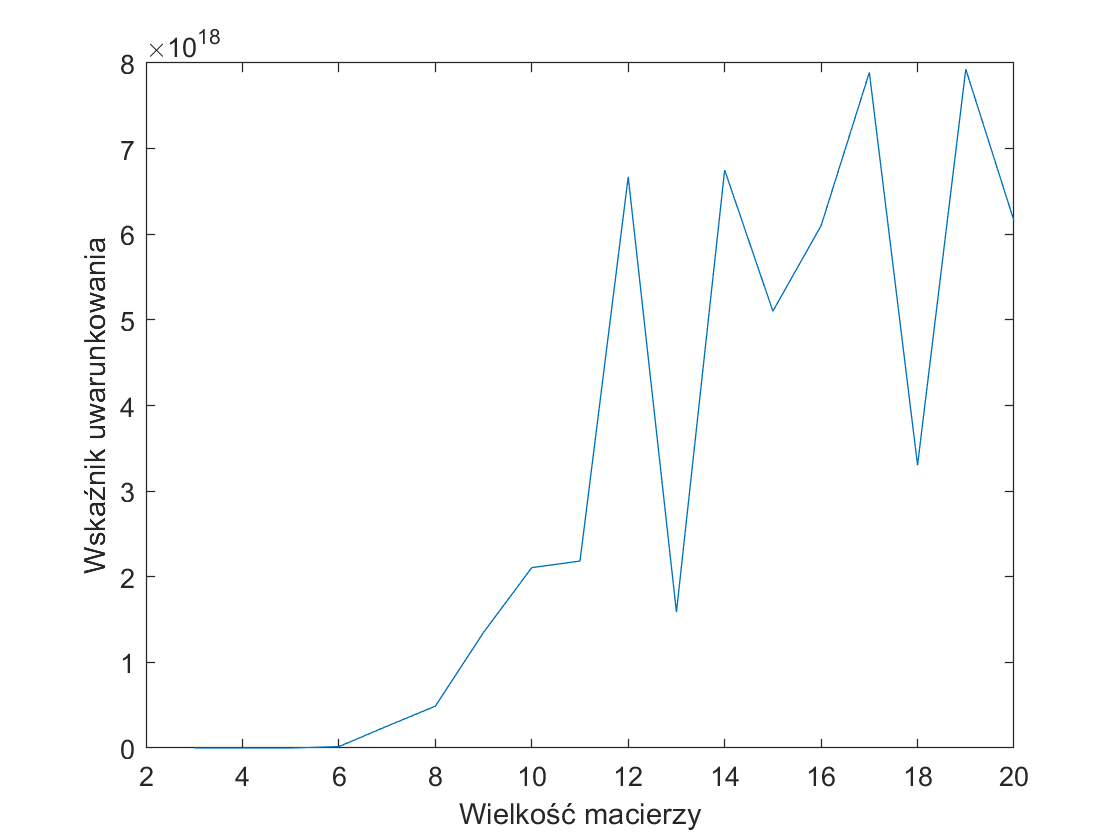
\includegraphics[width=10cm]{nphilb.eps}
\vskip-1.5ex
\caption{\footnotesize Zale\.zno\'s\'c wska\'znika uwarunkowania macierzy Hilberta od wymiar\'ow macierzy}
\label{npcondHilbert}
\end{figure}

Na powy\.zszych wykresach mo\.zemy dostrzec tendencj\k{e} do liniowego wzrostu wska\'znika uwarunkowania Macierzy Magicznej dla n nieparzystego. Natomiast dla n parzystego warto\'sci wska\'znika uwarunkowania zmieniaj\k{a} si\k{e} w spos\'ob znaczny malej\k{a}c, by dla kolejnej warto\'sci zn\'ow wzrosn\k{a}\'c. To mo\.ze by\'c przyczyn\k{a} nag\l{}ego wzrostu b\l{}\k{e}d\'ow dla n wi\k{e}kszego od 9.
\\
Z wykres\'ow ukazuj\k{a}cych zale\.zno\'s\'c mi\k{e}dzy wsp\'o\l{}czynnikiem stabilno\'sci, a wielko\'sci\k{a} macierzy Hilberta mo\.zna wywnioskowa\'c, \.ze zmiana wsp\'o\l{}czynnika stabilno\'sci nie zale\.zy od parzysto\'sci wymiar\'ow macierzy. Widzimy r\'ownie\.z tendencj\k{e} do zbli\.zania si\k{e} warto\'sci tego wsp\'o\l{}czynnika do zera dla coraz wi\k{e}kszych n.
\\
Analizuj\k{a}c b\l{}\k{e}dy mi\k{e}dzy wyznacznikiem obliczonym funkcj\k{a} detmd a det, dochodzimy do wniosku, \.ze wielko\'s\'c b\l{}\k{e}du w spos\'ob \'scis\l{}y zale\.zy od wska\'znika uwarunkowania macierzy oraz dodatkowo dla Macierzy Magicznej od jej wielko\'sci - dla n wi\k{e}kszych od 9 b\l{}\k{a}d drastycznie ro\'snie. 
\\
Natomiast dla funkcji invmd oraz inv mo\.zemy spostrzec wypisanie przez program ostrze\.zenia o wyznaczniku macierzy bliskiemu warto\'sci 0 dla macierzy Hilberta o wymiarach $7\times 7$, co zwraca nam uwag\k{e} na mo\.zliwe b\l{}\k{e}dy dla macierzy o niewielkich warto\'sciach wyznacznika. Jednak dla badanych warto\'sci n b\l{}\k{e}dy mi\k{e}dzy wynikami otrzymanymi tymi dwoma funkcjami s\k{a} niezauwa\.zalne bez dog\l{}\k{e}bniejszej analizy. 



\tableofcontents
\end{document}